While chapter~\ref{chap:language} gives a complete formal specification of the Evolog language extension, this chapter describes an implementation of said specification based on the Alpha \gls{asp} solver. All code referenced in this chapter is available on the official Github repository for Alpha~\cite{evolog-pr}.
\todo{in appendix, reference a git tag with alpha version of final thesis state that can run everything in here -- we wanna do this reproduceably!}

\section{Architectural overview of Alpha}
\label{sec:alpha-arch-overview}
\todo{maybe move this section to preliminaries}

Alpha is a lazy-grounding \gls{asp} solver implemented in Java. In a nutshell, Alpha calculates Computation Sequences (see Definition~\ref{def:prelims-asp-semantics-compseq}) for an input program using a \gls{cdnl}-inspired solving algorithm. Starting from the set of facts contained in the program, an initial truth assignment is constructed. Based on this assignment, ground instances are calculated for all rules that \emph{could potentially fire} based on the assignment. These ground instances are converted into \emph{noGoods} and passed to the solver component which, using an adapted \gls{cdnl} approach, guesses a new assignment based on the last set of noGoods. This process is repeated until no more guesses are possible, at which point the current assignment is either returned as an answer set, or some conflict is detected, in which case a new noGood is learned, and the solver backtracks. However, the actual ground-solve-loop is - while arguably at the heart of Alpha - just a small part of the process through which programs get evaluated. Figure \ref{fig:alpha-arch} gives an overview of the building blocks making up the Alpha system.\todo{cite alpha paper here}

\begin{figure}[t]
    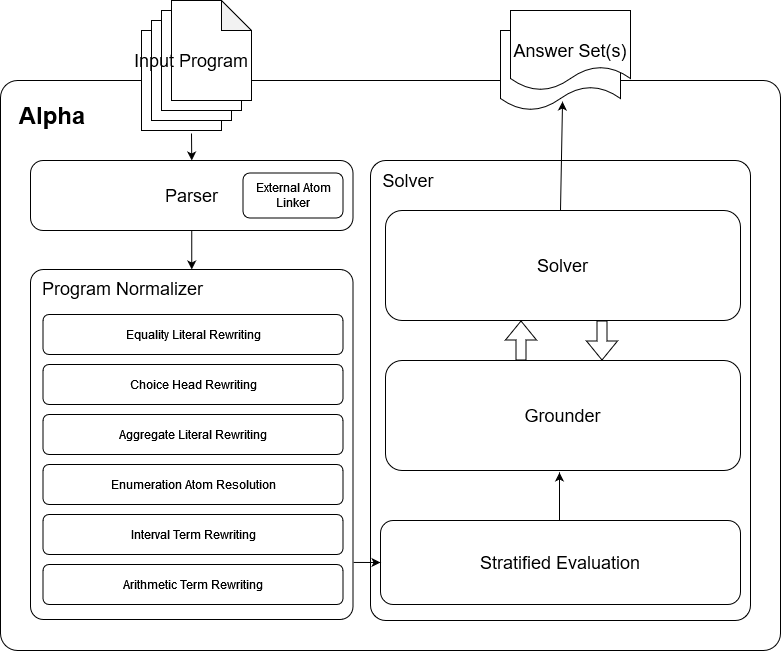
\includegraphics[width=\linewidth]{graphics/alpha-architecture.drawio.png}
    \caption{Alpha System Architecture}
    \label{fig:alpha-arch}
\end{figure}

\subsection{Parsing and Compilation}
\label{subsec:alpha-arch-compilation}

The core ground-and-solve component of Alpha supports only a subset of the input language described in Section~\ref{subsec:prelims-asp-syntax}. All language features supported by the parser, but not the solver itself, get compiled into equivalent constructs in the solver's internal representation. The following transformations are applied:
\begin{itemize}
    \item \emph{External Atom Linking}: Programs may only use external atoms whose implementations are known to the parser prior to parsing. Alpha provides a set of frequently used built-in external atoms out of the box, user-supplied code must be scanned through Alpha's API. Example~\ref{ex:user-supplied-externals} demonstrates the use of user-supplied atom definitions. All external atom implementations are linked during parsing, i.e. every external atom in the parsed program holds a reference to the implementing Java Method.
    \item \emph{Equality Literal Rewriting}: Literals like $A = B$ in rule bodies that establish an equality between variables are removed by replacing one variable with the other (e.g. $B$ with $A$ in the example). 
    \item \emph{Choice Head Rewriting}: Rules with a choice head get replaced by a set of rules and constriants that is semantically equivalent to the choice rule.
    \item \emph{Aggregate Literal Rewriting}: Aggregate literals like \texttt{N = \#count\{ X : interesting(X)\}} are replaced by a regular literal and a set of rules deriving instances of the replacement literal equivalent to the original aggregate literal. Subsection~\ref{subsubsec:alpha-arch-aggregate-rewriting} goes into more detail on the rewriting process.
    \item \emph{Enumeration Atom Resolution}: Alpha provides a feature where terms can be enumerated, i.e. the solver maps user-supplied terms to integers. This is used internally for Aggregate Literal Rewriting. Section~\ref{subsubsec:alpha-arch-enum-resolution} describes how the atoms in question are resolved.
    \item \emph{Interval Term Rewriting}: Interval terms, i.e. terms of form $A..B$ are transformed into regular variables that are bound through special internal literals which supply all values of the interval as ground instances of the variable.
    \item \emph{Arithmetic Term Rewriting}: In order to simplfy grounding later, terms constituting arithmetic expressions such as $p(f(X * 3, Y - 4))$ are rewritten such that no arithmetic expressions occur in nested terms, i.e. the atom from before would be rewritten to $p(f(R1, R2)), R1 = X * 3, R2 = Y - 4$.
\end{itemize}
The result of the above list of transformations is what is called a \emph{normalized} program in Alpha, which can directly be passed to the evaluation component and solved. Rewriting of Aggregate Literals and Resolution of Enumeration Atoms are of interest in the context of the Evolog reference implementation, and shall therefore be described in more detail.

\subsubsection{Enumeration Atoms}
\label{subsubsec:alpha-arch-enum-resolution}
Alpha permits use of an "enumeration" solver directive, which allows programs to associate terms with consecutive integer keys.
Listing~\ref{lst:enum-usage} demonstrates using an enumeration to assign integer ordinals to a set of colors. 
\begin{lstlisting}[style=asp-code, label={lst:enum-usage}, caption={Using the Enumeration Directive to enumerate color symbols.}]
#enumeration_predicate_is ordinal.

color(white). color(red). color(magenta).
color(yellow). color(green). color(cyan).
color(blue). color(black).
    
numbered_color(COL, NUM) :- 
    color(COL), ordinal(colors, COL, NUM).    
\end{lstlisting}    
The directive \texttt{\#enumeration\_predicate\_is} designates the predicate \texttt{ordinal/3} as an \emph{Enumeration Predicate}. All occurrences of the an enumeration predicate get replaced with a special internal predicate \texttt{\_Enumeration/3}. Listing~\ref{lst:enum-rewritten} shows the program from before after transformation.
\begin{lstlisting}[style=asp-code, label={lst:enum-rewritten}, caption={Transformed color numbering.}]
color(white). color(red). color(magenta).
color(yellow). color(green). color(cyan).
color(blue). color(black).

numbered_color(COL, NUM) :- 
    color(COL), _Enumeration(colors,COL,NUM).
\end{lstlisting} 
Alpha's grounding component calculates valid ground substitutions for enumeration atoms as follows: \\
Given an enumeration atom $a_e$ with terms $t_{enum}, t_{value}$ and $t_{ord}$ and a partial substitution $\sigma$, assigning ground values to $t_{enum}$ and $t_{value}$,
\begin{itemize}
    \item If the value $\sigma t_{enum}$ is encountered for the first time, initialize a new empty map (i.e. set of pairs with unique first elements), and associate it with  term $\sigma t_{enum}$.
    \item If the map for $\sigma t_{enum}$ does not contain a mapping for key $\sigma t_{value}$, extend $\sigma$ by the mapping $t_{ord} \mapsto o$, where $ = s + 1$ and $s$ denotes the current map size for $\sigma t_{enum}$. Add the mapping $(\sigma t_{ord}, o)$ to the map and return the extended version of $\sigma$.
    \item If a mapping for $\sigma t_{enum}$ and $\sigma t_{value}$ exists, read the associated ordinal $o$, add it to $\sigma$ and return the extended substitution.
\end{itemize}    
From a semantics point of view, enumeration literals can intuitively be seen as "lazily assigned fixed-interpretation literals"  (see Definition~\ref{def:prelims-asp-semantics-fixedinterpretation-literals}) in the way that every enumeration atom is true for exactly the ground substitution generated upon grounding it for the first time.
\todo{show the answer set}

\subsubsection{Aggregate Atoms}
\label{subsubsec:alpha-arch-aggregate-rewriting}

Alpha supports \emph{Aggregate Listerals} as defined in~\cite[p.~3]{asp-core2} by rewriting programs containing aggregate literals into sematically equivalent aggregate-free programs. A detailed description of Alpha's implementation of Aggregate Rewriting is available at~\cite{alpha-aggregate-support}, but would exceed the scope of this Thesis. We will therefore focus on general concepts applying to all aggregate functions that are rewritten, and outline the rewriting procedure for aggregate literals where the minimum or maximum over a set of terms is calculated, which is the starting point for compilation of the newly introduced $\#list$ aggregate described in Section~\ref{def:list-aggregation}.

In the context of this section, we consider literals of form $X \odot \#\mathit{func}\{t_1,\ldots,t_n : l_1,\ldots,l_m\}$, where $X$ is a term, $\odot \in \{=,\leq\}$ and $\mathit{func} \in \{\mathit{min},\mathit{max}\}$, $t_1,\ldots,t_n$ are terms and $l_1,\ldots,l_m$ literals, respectively.

\begin{definition}[Aggregate Terms, Elements, Local and Global Variables, Dependencies]
In the following, we use the notation $var(l_1,\ldots,l_n)$ for literals $l_1,\ldots,l_n$ to denote the set of variable terms occuring in said literals. Consider a rule $r$ containing aggregate literal $l_{agg} =  X \odot \#\mathit{func}\{t_1,\ldots,t_n : l_1,\ldots,l_m\}$:
\[
    H \leftarrow l_{agg}, b_1,\ldots,b_k.
\]
Then, the set $var(l_1,\ldots,l_n) \cap var(b_1,\ldots, b_k)$ is called \emph{global variables} of $l_{agg}$, denoted $glob(l_{agg})$. Roughly speaking, global variables of an aggregate literal are all variables occurring within the aggregate literal as well as other body literals of $r$. Given a set $V = glob(l_{agg})$, the set of literals $dep(l_{agg})$ is the mnimal set of literals that, given a substitution $\sigma$, must be ground after application of $\sigma$, in order for $\sigma$ to also ground $l_{agg} \cup dep(l_{agg})$.
Intuitively, global variables of an aggregate literals are all variables for which Alpha's lazy grounding component needs a ground value, in order to be able to calculate a ground instance of the aggregate literal itself. Dependencies of an aggregate literal $l_{agg}$are all literals of which the grounder needs ground instances in order to calculate a grounding of all global variables of $l_{agg}$.
\end{definition} 

In order to translate a rule $r$ containing an aggregate literal $l_{agg} = X \odot \#\mathit{func}\{t_1,\ldots,t_n : l_1,\ldots,l_m\}$ with global variables $glob(l_{agg})$, dependencies $dep(l_{agg})$ into a semantically equivalent set of rules, the following steps are taken:
\begin{itemize}
    \item Generate a unique identifier $id(l_{agg})$ (typically some integer) for $l_{agg}$
    \item Construct rule $r´$ in which $l_{agg}$ is replaced by a literal $aggregate\_result(id(l\_{agg})\_args, X)$
    \item Generate an \emph{element rule} which derives one atom per element that is being aggregated over. Given the aggregate element $t_1,\ldots,t_n : l_1,\ldots,l_m$, the corresponding element rule is $id(l_{agg})\_element\_tuple(id(l\_{agg})\_args, t_1,\ldots,t_n) \leftarrow l_1,\ldots,l_m, dep(l_{agg})$, i. e. the element rule body consists of all literals of the aggregate element together with all dependencies of the aggregate literal.
    \item Generate a set of \emph{encoding rules} that encode the actual aggregate function over all elements as derived by the element rule and derives instances of the $aggregate\_result/2$ predicate.
\end{itemize}     

Example~\ref{ex:aggregate-rewriting-min} demonstrates how an aggregate literal for the minimum function gets rewritten by Alpha.

\begin{example}
\label{ex:aggregate-rewriting-min}
Consider the program from Listing~\ref{lst:aggregate-rewriting-min-source}. Based on some facts of type $employee/3$ which assert that an employee works in some department and earns a given salary, we use a $\#min$-aggregate to find the employee with the lowest salary in each department.
\begin{lstlisting}[style=asp-code, label={lst:aggregate-rewriting-min-source}, caption={ASP program to find the worst paid employee per department.}]
employee(bob, sales, 2000).
employee(alice, development, 6000).
employee(dilbert, development, 4500).
employee(jane, sales, 3500).
employee(carl, controlling, 5000).
employee(bill, controlling, 4000).
employee(claire, development, 5000).
employee(mary, sales, 3000).
employee(joe, controlling, 5500).
    
department(DEP) :- employee(_, DEP, _).
    
min_salary(SAL, DEP) :- 
    SAL = #min{S : employee(_, DEP, S)}, 
    department(DEP).
worst_paid(DEP, EMP) :- 
    min_salary(S, DEP), employee(EMP, DEP, S).    
\end{lstlisting} 
Listing~\ref{lst:aggregate-rewriting-min-rewritten} shows a rewritten version of the original program.
\begin{lstlisting}[style=asp-code, label={lst:aggregate-rewriting-min-rewritten}, caption={The program from Listing~\ref{lst:aggregate-rewriting-min-source} in its rewritten version.}]
employee(bob, sales, 2000).
employee(alice, development, 6000).
employee(dilbert, development, 4500).
employee(jane, sales, 3500).
employee(carl, controlling, 5000).
employee(bill, controlling, 4000).
employee(claire, development, 5000).
employee(mary, sales, 3000).
employee(joe, controlling, 5500).

department(DEP) :- employee(_0, DEP, _1).
worst_paid(DEP, EMP) :- 
    min_salary(S, DEP), employee(EMP, DEP, S).
min_salary(SAL, DEP) :- 
    min_1_result(min_1_args(DEP), SAL), department(DEP).
min_1_element_tuple_less_than(ARGS, LESS, THAN) :- 
    min_1_element_tuple(ARGS, LESS), 
    min_1_element_tuple(ARGS, THAN), LESS <THAN.
min_1_element_tuple_has_smaller(ARGS, TPL) :- 
    min_1_element_tuple_less_than(ARGS, _3, TPL).
min_1_min_element_tuple(ARGS, MIN) :- 
    min_1_element_tuple(ARGS, MIN), 
    not min_1_element_tuple_has_smaller(ARGS, MIN).
min_1_result(ARGS, M) :- 
    min_1_min_element_tuple(ARGS, M).
min_1_element_tuple(min_1_args(DEP), S) :- 
    employee(_2, DEP, S), department(DEP).
\end{lstlisting}   
In the rewritten version, the rule in line 14, which derives $\mathit{min\_salary/2}$ has the aggregate literal replaced with a regular literal, instances for which are derived by newly added rules that together encode the aggregate function. 
The individual elements over which a minimum is being calculated are derived as instances of the \texttt{min\_1\_element\_tuple/2} predicate using the rule in line 26. In order to find the minimal instance of \texttt{min\_1\_element\_tuple/2}, we first establish a "less than"-relation (i.e. a partial order based on numeric comparison of the second term of the element tuple instances) using the rule in line 16. The minimum element is then the one for which we cannot find a "smaller" element. This element is derived by the rule in line 21.
The single answer set of the rewritten program (filtered for instances of \texttt{worst\_paid/2}) is $A =\{worst\_paid(controlling,bill),~worst\_paid(development,dilbert),~worst\_paid(sales,bob)\}$.
\end{example}    

\subsection{Evaluation}

Once a program has been parsed and compiled using the steps described in~\ref{subsec:alpha-arch-compilation}, the compiled program can be evaluated (i.e. solved). Evaluation consists of two steps - first, the stratified bottom (\emph{"common base program, CBP"},see~\ref{def:prelims-asp-semantics-cbp}) is evaluated using a bottom-up evaluation algorithm which is computationally more efficient than Alpha's \gls{cdnl}-based ground-/solve-loop.

\subsubsection{Stratified Evaluation in Alpha}

Based on a compiled program, $P_{comp}$

TODO: general outpline of evaluation with heavy focus on stratified evaluation, ground/solve loop is not of interest in this context, point to appropriate resources for that!

\section{Implementing the Evolog extension in Alpha}

TODO Architecture Diagram with added parts highlighted in color

\subsection{Implementing Action Support}

TODO

\subsection{Implementing Program Modularization}

Since, formally, module atoms are just a special type of external atoms, implementing support for Modularization as described in~\ref{sec:evolog-modules} mainly has to deal with how to parse module definitions and how to construct external atoms according to Alpha's internal representation from a set of parsed module definition for atoms which reference these definitions. While not strictly necessary, this section also discusses the newly added \texttt{\#list\{...\}} aggregate, which has been added as syntactic sugar for combining a set of terms into a single list term according to Definition~\ref{def:asp-list-term}.

\subsubsection{List aggregation}

External atoms are defined as having input- and output-\emph{terms} (but not multisets of terms). At the same time, it is self-evident that - in most cases - one has to pass multiple input facts to a module program - for instance, a graph has sets of edges and vertices, all of which need to be passed to a module dealing with graph problems. This is where lists come in. By establishing the convention that the \emph{single} input fact to a module program always has one or more \emph{list terms} as arguements, we are able to encode all information that needs to be passed to the module into a single atom, while still staying true to external atom semantics as supported by Alpha.
The parctical problem arising from this is that constructing list terms in ASP is rather cumbersome. One has to write rules to
\begin{itemize}
    \item specify \emph{what} goes into the list, i.e. one or more rules encoding eligible \emph{list elements},
    \item specify \emph{in what sequence} elements go into the list, i.e. rules which establish a total order between list elements,
    \item actually construct the list, i.e. starting from the end, recursively construct the term holding all list elements.
\end{itemize}
Listing~\ref{lst:graph-list-aggregation} shows an example of this approach, where a list term is constructed for vertices and edges of a graph, respectively.
\begin{lstlisting}[style=asp-code, label={lst:graph-list-aggregation}, caption={ASP code to create vertex and edge lists for a given graph.}]
%% pack vertices into a vertex list
vertex_element(E) :- vertex(E).
% First, establish ordering of elements
vertex_element_less(N, K) :- 
    vertex_element(N), vertex_element(K), N < K.
vertex_element_not_predecessor(N, K) :- 
    vertex_element_less(N, I), vertex_element_less(I, K).
vertex_element_predecessor(N, K) :- 
    vertex_element_less(N, K), 
    not vertex_element_not_predecessor(N, K).
vertex_element_has_predecessor(N) :- 
    vertex_element_predecessor(_, N).
% Now build the list as a recursively nested function term
vertex_lst_element(IDX, list(N, list_empty)) :- 
    vertex_element(N), 
    not vertex_element_has_predecessor(N), 
    IDX = 0.
vertex_lst_element(IDX, list(N, list(K, TAIL))) :- 
    vertex_element(N), 
    vertex_element_predecessor(K, N), 
    vertex_lst_elemen(PREV_IDX, list(K, TAIL)), 
    IDX = PREV_IDX + 1.
has_next_vertex_element(IDX) :- 
    vertex_lst_element(IDX, _), 
    NEXT_IDX = IDX + 1, 
    vertex_lst_element(NEXT_IDX, _).
vertex_lst(LIST) :- 
    vertex_lst_element(IDX, LIST), 
    not has_next_vertex_element(IDX).

%% pack edges into an edge list
edge_element(edge(V1, V2)) :- edge(V1, V2).
% First, establish ordering of elements
edge_element_less(N, K) :- 
    edge_element(N), edge_element(K), N < K.
edge_element_not_predecessor(N, K) :- 
    edge_element_less(N, I), edge_element_less(I, K).
edge_element_predecessor(N, K) :- 
    edge_element_less(N, K), 
    not edge_element_not_predecessor(N, K).
edge_element_has_predecessor(N) :- 
    edge_element_predecessor(_, N).
% Now build the list as a recursively nested function term
edge_lst_element(IDX, list(N, list_empty)) :- 
    edge_element(N), 
    not edge_element_has_predecessor(N), 
    IDX = 0.
edge_lst_element(IDX, list(N, list(K, TAIL))) :- 
    edge_element(N), 
    edge_element_predecessor(K, N), 
    edge_lst_element(PREV_IDX,list(K, TAIL)), 
    IDX = PREV_IDX + 1.
has_next_edge_element(IDX) :- 
    edge_lst_element(IDX, _), 
    NEXT_IDX = IDX + 1, 
    edge_lst_element(NEXT_IDX, _).
edge_lst(LIST) :- 
    edge_lst_element(IDX, LIST), 
    not has_next_edge_element(IDX).
\end{lstlisting} 
Given facts $vertex(a),~vertex(b),~vertex(c),~edge(a,b),~edge(b,c),~edge(c,a)$, we get the following answer set (filtered for predicates $edge\_lst/1$ and $vertex\_lst/1$) $A = \{edge\_lst(list(edge(c,a), list(edge(b,c), list(edge(a,b), list\_empty)))), vertex\_lst(list(c, list(b,list(a,list\_empty))))\}$

Considering Listing~\ref{lst:graph-list-aggregation}, it is easy to see that construction of a list term looks always the same, regardless of the actual elements going into the list. Furthermore, we can observe a distinct similarity to the code generated to rewrite a $\#min$-aggregate outlined in Section~\ref{subsubsec:alpha-arch-aggregate-rewriting}. In the following, we define a new aggregate function, $\#list$, which Alpha rewrites into a generalized version of the list encoding from Listing~\ref{lst:graph-list-aggregation}.

\begin{definition}[List Aggregate]
\label{def:list-aggregate}    
A \emph{list aggregate} is an aggregate atom of the following form
\[
    t_{res} = \#list\{ t_{elem} : l_{1},\ldots,l_{n}\}
\]
where $t_{res}$ and $t_{elem}$ are terms called result- and element-term, respectively, and $l_{1},\ldots,l_{n}$ are literals.
\end{definition}    
Definition~\ref{def:list-aggregate} formally defines the syntax of a list aggregate. Note that - in contrast to genral aggregate atoms, only equality comparisons, i.e. $X = \#list\{...\}$, are allowed, and we permit only a single element term rather than arbitrary tuples. Listing~\ref{lst:graph-list-aggregation-lstagg} shows a much shorter version of the program from Listing~\ref{lst:graph-list-aggregation}, in which list aggregation is used instead of step-by-step construction of list terms.
\begin{lstlisting}[style=asp-code, label={lst:graph-list-aggregation-lstagg}, caption={Creating vertex- and edge-lists using list aggregates.}]
%% pack vertices into a vertex list
vertex_lst(LIST) :- 
    LIST = #list{V : vertex(V)}.
    
%% pack edges into an edge list
edge_lst(LIST) :- 
    LIST = #list{edge(V1, V2) : edge(V1, V2)}.    
\end{lstlisting}

In order to compile list-aggregates into their semantically equivalent aggregate-free versions, the following handling of list aggregates has been added to ALpha's aggregate rewriting logic:
\begin{itemize}
    \item Substitute list aggregates in rules according to the general rules for aggregates outlined in~\ref{subsubsec:alpha-arch-aggregate-rewriting}.
    \item Element rules for list aggregates get constructed the same as for other aggregates, but permit only one element term rather than a tuple.
    \item In order to encode list construction, rules are added to construct a total order over all elements that should go into the list.
    \item List construction starts with the last element, which is defined to be the maximum element of the constructed order, successor elements are rcursively added to the front of the list.
    \item The list is complete when a list has been constructed, such that there is no element smaller than the current head of the list.
\end{itemize}
Listing~\ref{lst:graph-list-aggregation-rewritten} shows the rewritten version of the program form Listing~\ref{lst:graph-list-aggregation-lstagg} (Note that in the hand-crafted example from Listing~\ref{lst:graph-list-aggregation}, lists are constructed in descending element order, rather than ascending as is the case for the aggregate-based version).
\begin{lstlisting}[style=asp-code, label={lst:graph-list-aggregation-rewritten}, caption={Rewritten list aggregates from Listing~\ref{lst:graph-list-aggregation-lstagg}}]  
vertex_lst(LIST) :- 
    list_1_result(list_1_no_args, LIST).
edge_lst(LIST) :- 
    list_2_result(list_2_no_args, LIST).
list_1_element_greater(ARGS, N, K) :- 
    list_1_element(ARGS, N), 
    list_1_element(ARGS, K), 
    N > K.
list_1_element_not_successor(ARGS, N, K) :- 
    list_1_element_greater(ARGS, N, I), 
    list_1_element_greater(ARGS, I, K).
list_1_element_successor(ARGS, N, K) :- 
    list_1_element_greater(ARGS, N, K), 
    not list_1_element_not_successor(ARGS, N, K).
list_1_element_has_successor(ARGS, N) :- 
    list_1_element_successor(ARGS, _0, N).
list_1_lst_element(ARGS, IDX, lst(N, lst_empty)) :- 
    list_1_element(ARGS, N), 
    IDX = 0,
    not list_1_element_has_successor(ARGS, N).
list_1_lst_element(ARGS, IDX, lst(N, lst(K, TAIL))) :- 
    list_1_element(ARGS, N),
     list_1_element_successor(ARGS, K, N), 
     list_1_lst_element(ARGS, PREV_IDX, lst(K, TAIL)), 
     IDX = PREV_IDX + 1.
list_1_has_next_element(ARGS, IDX) :- 
    list_1_lst_element(ARGS, IDX, _1), 
    NEXT_IDX = IDX + 1, 
    list_1_lst_element(ARGS, NEXT_IDX, _2).
list_1_result(ARGS, LIST) :- 
    list_1_lst_element(ARGS, IDX, LIST), 
    not list_1_has_next_element(ARGS, IDX).
list_1_element(list_1_no_args, V) :- 
    vertex(V).
list_2_element_greater(ARGS, N, K) :- 
    list_2_element(ARGS, N), 
    list_2_element(ARGS, K), 
    N > K.
list_2_element_not_successor(ARGS, N, K) :- 
    list_2_element_greater(ARGS, N, I), 
    list_2_element_greater(ARGS, I, K).
list_2_element_successor(ARGS, N, K) :- 
    list_2_element_greater(ARGS, N, K), 
    not list_2_element_not_successor(ARGS, N, K).
list_2_element_has_successor(ARGS, N) :- 
    list_2_element_successor(ARGS, _3, N).
list_2_lst_element(ARGS, IDX, lst(N, lst_empty)) :- 
    list_2_element(ARGS, N), 
    IDX = 0, 
    not list_2_element_has_successor(ARGS, N).
list_2_lst_element(ARGS, IDX, lst(N, lst(K, TAIL))) :- 
    list_2_element(ARGS, N), 
    list_2_element_successor(ARGS, K, N), 
    list_2_lst_element(ARGS, PREV_IDX, lst(K, TAIL)), 
    IDX = PREV_IDX + 1.
list_2_has_next_element(ARGS, IDX) :- 
    list_2_lst_element(ARGS, IDX, _4), 
    NEXT_IDX = IDX + 1, 
    list_2_lst_element(ARGS, NEXT_IDX, _5).
list_2_result(ARGS, LIST) :- 
    list_2_lst_element(ARGS, IDX, LIST), 
    not list_2_has_next_element(ARGS, IDX).
list_2_element(list_2_no_args, edge(V1, V2)) :- 
    edge(V1, V2).   
\end{lstlisting}    

\subsubsection{Parsing Module Definitions}

Module definitions are parsed together with regular ASP code. Given a file containing a set of facts and rules and an arbitrary number of module definitions, Alpha's parser will group all rules and facts outside any module definition into one ASP program (i.e. the "main program"), and emit a set containing all encountered module definitions alongside with the parsed main program. Definition~\ref{def:module-definition-technical} details the technical representation of a module definition (which is basically a data structure storing all elements specified in the syntactical definition of a module, see~\ref{def:module-definition}). The actual code used in Alpha for parsing and storing module definitions can be found in the Appendix, see Example~\ref{ex:alpha-module-parsing}.

\begin{definition}[Internal module representation]
\label{def:module-definition-technical}
A parsed module definition gets stored as a tuple $M = (\mathit{name},\mathit{p_{in}},\mathit{OUT},\mathit{PROG})$ where
\begin{itemize}
    \item $\mathit{name}$ is a string representing the name of the module. This must be unique, i.e. Alpha currently has no concept of namespaces or similar means of distinguishing equally named modules,
    \item $\mathit{p_{in}}$ is a predicate (represented as a string of form $\mathit{name}/\mathit{arity}$) called \emph{input specification},
    \item $\mathit{OUT}$ denotes a (possibly empty) set of predicates called \emph{output specification},
    \item and $\mathit{PROG}$ is the ASP program holding the actual implementation code for the module.
\end{itemize}
\end{definition}   

\subsubsection{Module Literal Compilation}

Once a program and all contained module definitions have been parsed, every module atom (i.e. call to a module from a rule body) needs to be linked to its implementation. In Alpha, external atoms are evaluated during grounding. Definition~\ref{def:external-atom-interpretation} formally defines the notion of an \emph{external predicate interpretation}, i.e. an interpretation function for ground instances of external atoms. 

\begin{definition}[External Predicate Interpretation]
\label{def:external-atom-interpretation}    
 Given an external atom $\&\mathit{ext}[i_1,\ldots,i_n](o_1,\ldots,o_m)$ with input terms $i_1,\ldots,i_n$ and output terms $o_1,\ldots,o_m$, and a substitution $\sigma$ assigning ground values to at least all input terms of $ex$, the \emph{predicate interpretation function} $f: HU^n \mapsto 2^{HU^m}$ is a function which, for a given $n$-tuple over the Herbrand Universe $HU$, returns all $m$-tuples over $HU$ for which the ground atom $\&\mathit{ext}[\sigma(i_1),\ldots,\sigma(i_n)](r_1,\ldots,r_m)$ where $(r_1\ldots,r_m) \in f(\sigma(i_1),\ldots,\sigma(i_n))$ is true.
\end{definition}

Implementation-wise, predicate interpretations are Java methods with a specific signature. Listing~\ref{lst:predicate-interpretation-interface} shows the corrseponding interface definition. Note that, for an implementation of \texttt{PredicateInterpretation} to be valid, it must be pure functional, i.e. not have any side-effects.
\begin{lstlisting}[style=java, label={lst:predicate-interpretation-interface}, caption={Java Interface for Predicate Interpretations}]
@FunctionalInterface
public interface PredicateInterpretation {
    
    Set<List<Term>> evaluate(List<Term> terms);

}    
\end{lstlisting}

\paragraph{Constructing interpretations for Module Atoms}
Listing~\ref{lst:module-interpretation-impl} shows the (abbreviated) Java code used in Alpha to construct a \texttt{PredicateInterpretation} for a module atom. Boundary checks and similar validations as well as auxiliary method calls are left out for easier readability. The interpretation itself is constructed using the Lambda-expression \texttt{PredicateInterpretation interpretation = terms -> \{...\}}, where \texttt{terms} is the list of input terms, which gets wrapped into an atom of the predicate defined in \texttt{inputSpec} (i.e. the module input specification). Answer sets get filtered based on predicate names according to the module's output specification. Finally, each answer set is converted to a list of list terms using function \texttt{answerSetToTerms}, and the resulting set of term lists is returned.
\begin{lstlisting}[style=java, label={lst:module-interpretation-impl}, caption={Constructing module interpretations}]
private ExternalAtom translateModuleAtom(ModuleAtom atom, Map<String, Module> moduleTable) {
    ...
    Predicate inputSpec = definition.getInputSpec();
    ...
    Set<Predicate> outputSpec = definition.getOutputSpec();
    Set<Predicate> expectedOutputPredicates;
    if (outputSpec.isEmpty()) {
    	expectedOutputPredicates = calculateOutputPredicates(normalizedImplementation);
    } else {
    	expectedOutputPredicates = outputSpec;
    }
    ...
    PredicateInterpretation interpretation = terms -> {
    	BasicAtom inputAtom = Atoms.newBasicAtom(inputSpec, terms);
    	NormalProgram program = Programs.newNormalProgram(
            normalizedImplementation.getRules(),
    		ListUtils.union(List.of(inputAtom), 
            normalizedImplementation.getFacts()), 
            normalizedImplementation.getInlineDirectives(), 
            Collections.emptyList());
    	java.util.function.Predicate<Predicate> filter = outputSpec.isEmpty() ? p -> true : outputSpec::contains;
    	Stream<AnswerSet> answerSets = moduleRunner.solve(program, filter);
    	if (atom.getInstantiationMode()
            .requestedAnswerSets().isPresent()) {
    		answerSets = answerSets.limit(
                atom.getInstantiationMode()
                    .requestedAnswerSets().get());
    	}
    	return answerSets.map(as -> answerSetToTerms(as, expectedOutputPredicates))
            .collect(Collectors.toSet());
    };
    return Atoms.newExternalAtom(atom.getPredicate(), interpretation, atom.getInput(), atom.getOutput());
}

private static List<Term> answerSetToTerms(AnswerSet answerSet, Set<Predicate> moduleOutputSpec) {
    List<Term> terms = new ArrayList<>();
    for (Predicate predicate : moduleOutputSpec) {
        if (!answerSet.getPredicates().contains(predicate)) {
            terms.add(Terms.EMPTY_LIST);
        } else {
            terms.add(Terms.asListTerm(
                    answerSet.getPredicateInstances(predicate).stream()
                        .map(Atoms::toFunctionTerm)
                        .collect(Collectors.toList())));
        }
    }
    return terms;
}
\end{lstlisting}    



\todo{need to decide whether module recursion is a thing! (probably should be)}
\section{Evolog applications}

TODO: A few programs using both actions and modules to achieve something cool!